%% This is file `sample-sigconf-authordraft.tex',
%% generated with the docstrip utility.
%%
%% The original source files were:
%%
%% samples.dtx  (with options: `all,proceedings,bibtex,authordraft')
%% 
%% IMPORTANT NOTICE:
%% 
%% For the copyright see the source file.
%% 
%% Any modified versions of this file must be renamed
%% with new filenames distinct from sample-sigconf-authordraft.tex.
%% 
%% For distribution of the original source see the terms
%% for copying and modification in the file samples.dtx.
%% 
%% This generated file may be distributed as long as the
%% original source files, as listed above, are part of the
%% same distribution. (The sources need not necessarily be
%% in the same archive or directory.)
%%
%%
%% Commands for TeXCount
%TC:macro \cite [option:text,text]
%TC:macro \citep [option:text,text]
%TC:macro \citet [option:text,text]
%TC:envir table 0 1
%TC:envir table* 0 1
%TC:envir tabular [ignore] word
%TC:envir displaymath 0 word
%TC:envir math 0 word
%TC:envir comment 0 0
%%
%% The first command in your LaTeX source must be the \documentclass
%% command.
%%
%% For submission and review of your manuscript please change the
%% command to \documentclass[manuscript, screen, review]{acmart}.
%%
%% When submitting camera ready or to TAPS, please change the command
%% to \documentclass[sigconf]{acmart} or whichever template is required
%% for your publication.
%%
%%
\documentclass[sigconf,authordraft]{acmart}
\usepackage{float}
\usepackage{placeins}
\title{Post CMOS technologies: An Overview and Analysis}
%%
%% \BibTeX command to typeset BibTeX logo in the docs
\AtBeginDocument{%
  \providecommand\BibTeX{{%
    Bib\TeX}}}

%% Rights management information.  This information is sent to you
%% when you complete the rights form.  These commands have SAMPLE
%% values in them; it is your responsibility as an author to replace
%% the commands and values with those provided to you when you
%% complete the rights form.
\setcopyright{acmlicensed}
\copyrightyear{2018}
\acmYear{2018}
\acmDOI{XXXXXXX.XXXXXXX}
%% These commands are for a PROCEEDINGS abstract or paper.
\acmConference[Conference acronym 'XX]{Make sure to enter the correct
  conference title from your rights confirmation email}{June 03--05,
  2018}{Woodstock, NY}
%%
%%  Uncomment \acmBooktitle if the title of the proceedings is different
%%  from ``Proceedings of ...''!
%%
%%\acmBooktitle{Woodstock '18: ACM Symposium on Neural Gaze Detection,
%%  June 03--05, 2018, Woodstock, NY}


%%
%% Submission ID.
%% Use this when submitting an article to a sponsored event. You'll
%% receive a unique submission ID from the organizers
%% of the event, and this ID should be used as the parameter to this command.
%%\acmSubmissionID{123-A56-BU3}

%%
%% For managing citations, it is recommended to use bibliography
%% files in BibTeX format.
%%
%% You can then either use BibTeX with the ACM-Reference-Format style,
%% or BibLaTeX with the acmnumeric or acmauthoryear sytles, that include
%% support for advanced citation of software artefact from the
%% biblatex-software package, also separately available on CTAN.
%%
%% Look at the sample-*-biblatex.tex files for templates showcasing
%% the biblatex styles.
%%

%%
%% The majority of ACM publications use numbered citations and
%% references.  The command \citestyle{authoryear} switches to the
%% "author year" style.
%%
%% If you are preparing content for an event
%% sponsored by ACM SIGGRAPH, you must use the "author year" style of
%% citations and references.
%% Uncommenting
%% the next command will enable that style.
%%\citestyle{acmauthoryear}


%%
%% end of the preamble, start of the body of the document source.
\begin{document}

%%
%% The "title" command has an optional parameter,
%% allowing the author to define a "short title" to be used in page headers.
\title{Post CMOS technologies: An Overview and Analysis}

%%
%% The "author" command and its associated commands are used to define
%% the authors and their affiliations.
%% Of note is the shared affiliation of the first two authors, and the
%% "authornote" and "authornotemark" commands
%% used to denote shared contribution to the research.
\author{Willson Luo}
\email{willsonluo@ucla.edu}
\affiliation{
  \institution{University of California Los Angeles}
  \city{Los Angeles}
  \state{California}
  \country{USA}
}

%%
%% By default, the full list of authors will be used in the page
%% headers. Often, this list is too long, and will overlap
%% other information printed in the page headers. This command allows
%% the author to define a more concise list
%% of authors' names for this purpose.
%%
%% The abstract is a short summary of the work to be presented in the
%% article.
\begin{abstract}
  The rapid evolution of computing is pushing the limits of traditional 
  silicon-based electronics, necessitating the exploration of 
  novel materials and architectural paradigms. This paper 
  investigates three transformative technologies poised to 
  redefine future computational systems: Carbon Nanotubes 
  (CNTs), Spintronics, and Memristors. We explore how Carbon 
  Nanotube Field-Effect Transistors (CNFETs) offer enhanced 
  performance and energy efficiency by enabling scaling beyond 
  conventional limits, exemplified by the development of 
  sophisticated CNFET-based microprocessors. Concurrently, 
  Spintronics, particularly through Magnetoelectric Spin-Orbit 
  (MESO) devices, promises ultra-low power logic by leveraging 
  electron spin, introducing innovative concepts like majority 
  logic gates. Furthermore, we examine Memristors, which address 
  the Von Neumann bottleneck by integrating memory and processing, 
  facilitating advanced applications in neuromorphic and analog 
  computing, as demonstrated by their use in artificial neural 
  networks and threshold logic gates. While each technology 
  presents unique challenges in fabrication and integration, 
  their distinct advantages offer compelling pathways toward 
  building faster, smaller, and more energy-efficient computing 
  systems for the next generation.
  CMOS.
\end{abstract}

%%
%% The code below is generated by the tool at http://dl.acm.org/ccs.cfm.
%% Please copy and paste the code instead of the example below.
%%
%%
%% Keywords. The author(s) should pick words that accurately describe
%% the work being presented. Separate the keywords with commas.
\keywords{Do, Not, Us, This, Code, Put, the, Correct, Terms, for,
  Your, Paper}
%% A "teaser" image appears between the author and affiliation
%% information and the body of the document, and typically spans the
%% page.

%%
%% This command processes the author and affiliation and title
%% information and builds the first part of the formatted document.
\maketitle

\section{Introduction}
The pursuit of faster, smaller, and more energy-efficient computing
has been a driving force for technological advancement since the 
creation of the transistor. For decades, CMOS (Complementary
metal-oxide-semiconductor) technology has served as the foundation 
of of the modern computer. However, as we continue to approve our 
transistors and approach fundamental limits, the need for novel 
paradigms becomes increasinly urgent. This paper explores three 
technologies that could shape the future of computing: Carbon Nanotubes
(CNTs), Spintronics, and Memristors. Each offers their own 
advantages that address the limitations of silicon transistors,
varying from faster performance to significantly reduced power 
consumption. 

Carbon Nanotubes, with their exceptional electrical and thermal 
properties, present a compelling alternative to silicon in 
field-effect transistors (FETs). The ability to scale devices 
beyond current limits, coupled with high carrier mobility and 
superior heat dissipation, positions Carbon Nanotube FETs (CNFETs) 
as a potential successor for high-performance, low-power logic. 
Recent advancements, such as the development of the RV16X-NANO 
microprocessor at MIT, demonstrate the practical viability of 
CNFET-based computing, showcasing their compatibility with 
existing design methodologies and their ability to execute 
complex instructions.

Beyond simply replacing silicon, Spintronics offers a 
revolutionary approach to information processing by leveraging 
the intrinsic spin of electrons in addition to their charge. 
Magnetoelectric Spin-Orbit (MESO) devices, a key development in 
spintronics, promise ultra-low power logic operations by directly 
coupling electron spin with its movement and enabling control 
through both electrical and magnetic properties. These devices 
offer superior switching energy, lower operating voltages, and 
enhanced logic density, with the potential to implement universal 
logic through majority gates, fundamentally transforming how logic 
functions are conceived and executed.

Finally, Memristors, often described as the "fourth fundamental 
circuit element," introduce a new dimension to computing by 
combining memory and processing capabilities within a single 
device. This integration directly addresses the Von Neumann 
bottleneck, the traditional separation of memory and logic that 
limits computational speed and efficiency. Memristor-based 
threshold logic gates and crossbar arrays hold immense promise 
for neuromorphic and analog computing, enabling highly efficient 
Vector-Matrix Multiplication (VMM) crucial for artificial neural 
networks. While challenges in manufacturing reliability and 
programmability persist, the ability of memristors to store 
multiple bits and their non-volatile nature offer a path toward 
more compact, power-efficient, and brain-inspired computing 
architectures.

This paper will delve into the principles, advancements, and 
challenges associated with each of these transformative technologies, 
highlighting their individual contributions and their collective 
potential to shape the next generation of computing systems.

\section{Carbon Nanotubes (CNTs) for Advanced Electronics}
As the semiconductor continues its pursuit of miniaturization 
and greater performance, the fundamental limits of silicon-based 
transistors become increasingly apparent. This fundamental limit to 
the scaling of traditional transistors has given rise to many 
alternatives among them being Carbon Nanotubes (CNTs), one 
dimensional nanostructures that possess a unique combination of 
characteristics making them highly attractive for advancing 
electronics.

CNTs are composed of graphene sheets rolled into cylindrical tubes
with their structure determining whether they behave as
semiconductors or metals. his tunable electrical property,
coupled with their nanoscale dimensions, 
high carrier mobility, and exceptional thermal conductivity, 
positions CNTs as a compelling material for high-performance 
computing. Their inherent flexibility also opens avenues for 
novel applications beyond traditional rigid electronics. 
This section will delve into the fundamental properties of 
CNTs, explore their application in Carbon Nanotube Field-Effect 
Transistors (CNFETs), highlight recent advancements that 
demonstrate their potential, and discuss the significant 
fabrication challenges that must be overcome for their widespread 
adoption.

\subsection{Fundamental Properties of Carbon Nanotubes}
Carbon nanotubes are made of an allotrope of carbon known as 
graphene.

Their structure can be characterized into to major types.
Single-walled and multi-walled carbon nanotubes. Single-walled 
carbon nanotubes consist of a single graphene sheet rolled into 
a cylinder typically with a diameter between 0.5 to 2.0 
nanometers. Multi-walled carbon nanotubes are comprised of 
multiple concentric graphene cylinders nested within each other. 
Their diameter can extend up to tens of nanometers. 

The electrical properties can also vary depending on the structure 
and chirality (the angle at which the graphene sheet
is rolled up) of the CNTs. This means that a CNT can behave either 
as metals with a high conductivity or semiconductors making them 
suitable for making transistors. 

CNTs also have extremely high thermal conductivity making them
suitable to overcome many of the power limitations of current 
CMOS scaling.

Finally, CNTs are among the strongest and stiffest materials 
known, possessing exceptional tensile strength and elastic 
modulus. Moreover, they are remarkably flexible, capable of 
withstanding considerable mechanical strain without fracturing. 
This flexibility is particularly advantageous for emerging 
flexible electronics and 3D integration. 

\subsection{Carbon Nanotube Field Effect Transistors (CNFETs)}
The ability of semiconductor CNTs to conduct extremely effectively 
and their nanoscale dimensions make them ideal candidates for 
making the channel in field effect transistors. These properties 
allow CNFETs to offer several significant advantages over silicon 
based FETs:
\begin{itemize}
  \item Aggressive Scaling: Their nanoscale dimensions allow for
  device scaling below the 5 nanometer limit.
  \item High Carrier Mobility: The ballistic or near-ballistic 
  transport of carriers within CNTs leads to very high carrier
  mobility, which translates directly to faster switching speeds 
  and improved device performance.
  \item Lower Power Consumption: CNFETs can operate effectively 
  at lower voltages due to their superior electrical 
  characteristics, resulting in significantly reduced power 
  dissipation.
  \item Enhanced Gate Control: As one-dimensional materials, 
  CNTs offer excellent electrostatic control by the gate, 
  leading to lower off-state currents and steeper subthreshold 
  swings.
  \item Superior Thermal Management: Their high thermal 
  conductivity facilitates efficient heat dissipation, 
  mitigating hot spots and improving reliability in densely 
  packed circuits.
  \item Material Flexibility: The mechanical flexibility of CNTs 
  enables the development of bendable electronics and facilitates 
  potential three-dimensional chip stacking and integration, 
  offering new avenues for compact and innovative designs.
\end{itemize}

\begin{figure}[h]
  \centering
  \includegraphics[width = \linewidth]{images/Screenshot 2025-05-26 at 8.51.02 PM.png}
  \caption{Diagram of CNFET as combination of MOSFET and FinFET}
\end{figure}

\subsection{Logic Operations}
Since CNFETs operate just like normal transistors their integration 
into creating logic gates is the exact same as a traditional 
transistor. They still follow CMOS architecture and their benefits 
come from their performance advantage compared to traditional transistors rather than 
new operating paradigms. 

\subsection{Recent Advancements: RV16X-NANO Microprocessor}
The RV16X-NANO Microprocessor has been one of the biggest advancements 
in making a computer with CNFETs. The MIT Medical Electronic Device 
Realization Center were able to develop a 16 bit nanoprocessor which
they named RV16X-NANO. The microprocessor was built of the RISC-V
instruction set which was written through Bluespec and then compiled 
into Verilog, an RTL hardware description langauge. The microprocessor 
was comprised of over 14000 CMOS CNFETs that were made using more than 
10 million CNTs. 

On this microprocessor they were able to implement many standard logic 
blocks like multiplexers, arithmetic logic units, decoders, and encoders. 
Most notably, they were able to execute the famous "Hello World"
program.

\begin{figure}
  \centering
  \includegraphics[width = \linewidth]{images/Screenshot 2025-05-26 at 8.56.27 PM.png}
  \caption{Architecture and Design of RV16X-NANO}
\end{figure}

\subsection{Challenges in CNFET Fabrication and Integration}
Despite the considerable amount of progress made, several challenges 
still need to be addressed before CNFETs can achieve widespread 
viability and meet yield requirements for very large scale integration
(VLSI). Most signficantly, material and manufacturing defects are 
the current biggest challenge. Current methods of CNT fabrication 
lack a reliable way of controlling the chirality leading to many
CNTs exhibiting metallic properties instead of being semiconductors. 
Even after achieving semiconducting CNTs, manufacturing processes still
introduce defects and variability across a wafer. This includes variation
in CNFET density and contact resistance leading to non uniform performance
across an entire chip. In addition to manufacturing issues there 
still lacks a way of seamlessly integrating with traditional silicon
CMOS components. Overcoming these challenges is crucial to achieving 

\subsection{Personal Thoughts}
Overall CNFETs seem like a very promising area where there could be 
a lot of development. Since it doesn't deviate signficantly from 
traditional transistors it can be implemented into already made 
computing schemes making it more appealing for companies to invest 
in. It is much more likely for top fabrication companies like 
TSMC or Intel to look into CNFETs than some other technologies
that present completely new computing paradigms. The progress made in 
CNFETs has also been extremely promising as demonstrated by MIT's 
RV16X-NANO computer. The milestone to already have demonstrated 
such funcionality proves that this is a technology that is really 
feasible for the future. Graphene is also an area that has a good 
amount of research going into it so carbon nanotubes in general 
are sure to get more attention. 

With new chips there is a greater emphasis on chiplet technology 
as well as 3D integration. Again, CNFETs look very promising in that
area. Along with that, the medical industry is also constantly looking 
for flexible devices that can better interact with the human body 
which is another area where CNFETs shine in. 

Though there are still some big hurdles to overcome in manufacturing 
CNFETs at large scales and reliably I believe with just a few more 
breakthroughs they can become quite mainstream where large amounts 
of investments will be poured into CNFETs and accelerate their development 
greatly. 

\section{Spintronics: Beyond Charge-Based Computing}
Traditional electronics primarily rely on the charge of electrons 
to process and store information. 1s and 0s are coded by high and 
low volages which are determined by electric fields created by
distributions of charges. However, this approach faces inherent 
limitations in terms of power consumption and switching speed as 
devices continue to shrink. Spintronics emerges as a new paradigm 
that seeks to overcome these limitations by exploiting not only electron's 
charge but also its intrinsic angular momentum, known as spin. 
This additional degree of freedom offers the potential for 
fundamentally new device functionalities, leading to 
ultra-low power consumption, higher operating speeds, and increased 
logic density.

\subsection{Introduction to Spintronics}
Spintronics is the study and exploitation of the spin 
of electrons in solid-state devices. Unlike charge, which is a 
scalar quantity, spin is a quantum mechanical property that can 
be oriented in different directions (e.g., "spin-up" or "spin-down").
This allows for the encoding of information in a non-volatile magnetic
state. The promise of spintronics lies in its ability to enable 
novel functionalities and overcome the inherent energy dissipation 
associated with moving charges in conventional electronics. By manipulating 
spin currents and magnetic states, spintronic devices aim to perform logic 
operations with significantly reduced energy footprints. 
By also utilizing using a charge as well as spin this gives the potential to encode more 
states where there can be a combination of high or low voltage along 
with up or down spin. 


\subsection{Magnetoelectric Spin-Orbit (MESO) Devices} 
One promising way to compute and perform logic using spintronics is 
Magnetoelectric Spin-Orbit (MESO). In this scheme binary is represented 
in the up or down spin state of a nanomagnet. These devices rely 
on 2 major physical effects. The first is spin-orbit transduction where 
if a current flows through a material with a strongly coupled spin 
the current will also gain that spin. The second effect is magnetoelectric 
switching where you can control a materials magnetic properties by applying 
an electric field. For instance switching the spin state with the help of 
an electric field.

\subsubsection{Principle of Operation}
An input logic is provided through a voltage and electric field which 
will set the magnetization in a magnet to be in a certain direction. This 
converts an electrical input into a magnetic state where the spin state 
can now be used to represent the binary 0 or 1. 

To then generate an output a current is injected into the nanomagnet 
which will cause the output current from the nanomagnet to all have 
the same 

\section{Memristors}
The Von Neumann architecture, which physically separates the processing 
unit from the memory has been the preferred method for making computers. 
However, as our chips become faster bottlenecks from I/O also come up 
where information can't be moved to and from the chip fast enough. Memristors, 
first described as the fourth missing circuit element, offer a way 
to link memory and compute in a single device. This combination opens up
potential for more efficient brain inspired computing, particularly 
in the neuromorphic and analog world. 

\subsection{The Memristor Concept}
A memristor, combination of the words memory and resistor, is a device 
that can have a programmble resistance. It was often described as 
the fourth circuit element because it was believed that magnetic fields 
could be used to change the resistance of these devices. However, recent 
devices don't rely on magnetic fields at all and instead use electric fields 
to change the physical and chemical properties of these devices to program 
the resistance. This property, where it can "remember" its resistance allows 
for non volatile memory and reconfigurable logic without having to change 
the physical connections on a chip.

In addition to these new computing regimes they also offer advantages 
in several other areas. They can be manufactured into nanoscale 
dimensions below those of a silicon transistor allowing for greater scaling 
and higher density integration. Their ability to store memory even 
when power is switched enables lower power consumption. Since they can 
also be programmed into continuous resistance values they have the 
ability to store more than just 1 bit per device. Recent experiments
have shown one memristor being able to store 5-7 bits. Advances 
in memristors have also demonstrated a high level of CMOS compatability 
allowing them to be used in hybrid structures with traditional CMOS 
devices. 

\subsection{Memristor Based Threshold Logic Gate (TLG)}
Beyond their abilities to store memory, memristors are perfectly suited 
for implementing threshold logic gates. 

\subsubsection{Threshold Logic Gate}
A threshold logic gate is a gate that outputs a high signal if 
an input signal surpasses a certain threshold and outputs low 
otherwise. To give an example simply, imagine the input had a range 
of voltages from 0-9 and there is a threshold voltage of 5. Any
input voltage above high will output a binary high signal from the 
gate and any voltage below will output a low signal. A TLG 
is oftentimes also used to analyze a weighted sum from its inputs 
and see if that is above the threshold. 

With these characteristics a TLG can implement any linearly separable
function. This means that for a given function, there exists a 
dividing line (or hyperplane in higher dimensions) that would 
separate all input combinations to one of two distinct output 
groups. 

This also means that a single TLG can implement a boolean function 
that would require multiple logic gates to realize. For example, a 
majority gate would require at least 4 NAND gates to be realized in 
traditional CMOS design while it can be implemented in just one TLG. 

\subsubsection{Memristor-Based Threshold Logic Gate}
Memristors are ideal for TLG implementation since their variable 
resistance can act as programmable weights. A common architecture
for a memristor based TLG implements a hybrid architecture with 
memristors and traditional CMOS components into two main parts:
a differential part and a sensor part. 

The differential part is where a memristor is actually used. Each 
memristor is paired with a transistor known as a 1T1M array.
Here an input and reference threshold signal is taken in. When a 
voltage is then applied as the input current flows through the
memristor. The memristor here acts as a knob that controls how much 
current is passed through this differential part. This part 
can also be switched off when not in use to save power. 

The current from the differential part then goes to the sensor. 
The sensor compares a combined current coming from either one or 
multiple differential parts and sees if its above the threshold. 
Based on this comparison either a 1 or 0 is outputted indicating 
whether the sum of the weights have surpassed the threshold. 
%\cite here%

\subsubsection{Challenges}
Despite the theoretical efficiency of memristor based TLGs, 
their practical implementation still face significant challenges. 
Fabrication is still very difficult and there are no EDA tools 
compatible with designing devices made of memristors TLGs. 

\subsection{Hardware Implementation of Memristor-Based Artificial Neural Networks}
Beyond logic gates, memristors are particularly compelling for 
neural networks due to their inherent ability to perform efficient 
vector matrix multiplicaton which serves as the backbone of 
modern neural networks. 

\subsubsection{Vector-Matrix Multiplication (VMM) Core}
The central component in the vector-matrix multiplication core 
is the memristor crossbar array. In this array, memrisotrs are placed
at the crosspoints of a grid of wires. Voltages are inputted through
the rows of the wire and the at each cross point the current is 
found through Ohm's Law. Kirchoff's current law then sums up all the 
currents through the vertical beams and the sum of these currents 
is the result of the vector multiplication. Mathematically the
product as a current is 
\[I_j = \Sigma_iV_iG_{ij}.\]

These raw analog values are then fed to a analog to digital converter
(ADC) to then turn into digital magnitudes. Finally, an activation
function (often a sigmoid or ReLU) is applied to these results to 
introduce nonlinearities, making the output resemble various desired 
distributions. 
\begin{figure}[H]
  \centering
  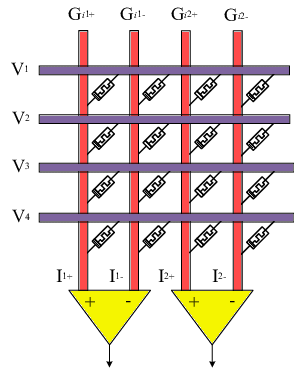
\includegraphics[scale = 0.3]{images/Neural-network-implementation-using-memristor-crossbar-arrays-a-shows-a-conventional.png}
  \caption{Memristor crossbar array}
\end{figure}

\subsubsection{Demonstrations of Memristor Neural Networks}
Notably, the University of Michigan created a memristor based 
computer that utilized a 54x108 memristor crossbar array. 
With this computer they were able to create a single layer perception 
that classified a 5x5 array of pixels, identifying the greek letters 
drawn in the 25 pixel array with 100\% accuracy. In addition, they 
implemented a two layer neural network that found commonalities and 
differences in breast cancer screenings, correctly classifying 
the cases as benign or malignant with 94.6\% accuracy.
%cite here%

\subsection{Challenges to Implementing Memristors}
Despite their demonstrated potential, several critical challenges still
prevent the widespread and practical use of memristors. Among these challenges
the most prominent ones are the lack of reliable manufacturing ability,
resistance drift, and non-linear resistance programming. 

Memristors are still unable to be manufactured reliably and the 
the cost of metal alloys is much more than that of silicon. Manufacturing 
metals to these scales is also much harder. These manufactured devices also 
suffer from drift where the programmed resistance can change over time 
to deviations in the environment like temperature. Non-linearities 
in how the resistance is programmed also make it extremely difficult to
program large scale memristor arrays. Supposed identitical memristors 
could require different voltage thresholds or to be applied for varying 
amount of times to program them to have the same resistance. 

\subsection{Personal Thoughts}
With the advent of 

\section{Comparative Analysis}

\section{Conclusion}

\section{Acknowledgments}

Authors of any work published by ACM will need to complete a rights
form. Depending on the kind of work, and the rights management choice
made by the author, this may be copyright transfer, permission,
license, or an OA (open access) agreement.

Regardless of the rights management choice, the author will receive a
copy of the completed rights form once it has been submitted. This
form contains \LaTeX\ commands that must be copied into the source
document. When the document source is compiled, these commands and
their parameters add formatted text to several areas of the final
document:
\begin{itemize}
\item the ``ACM Reference Format'' text on the first page.
\item the ``rights management'' text on the first page.
\item the conference information in the page header(s).
\end{itemize}

Rights information is unique to the work; if you are preparing several
works for an event, make sure to use the correct set of commands with
each of the works.

The ACM Reference Format text is required for all articles over one
page in length, and is optional for one-page articles (abstracts).

\section{CCS Concepts and User-Defined Keywords}

Two elements of the ``acmart'' document class provide powerful
taxonomic tools for you to help readers find your work in an online
search.

The ACM Computing Classification System ---
\url{https://www.acm.org/publications/class-2012} --- is a set of
classifiers and concepts that describe the computing
discipline. Authors can select entries from this classification
system, via \url{https://dl.acm.org/ccs/ccs.cfm}, and generate the
commands to be included in the \LaTeX\ source.

User-defined keywords are a comma-separated list of words and phrases
of the authors' choosing, providing a more flexible way of describing
the research being presented.

CCS concepts and user-defined keywords are required for for all
articles over two pages in length, and are optional for one- and
two-page articles (or abstracts).

\section{Sectioning Commands}

Your work should use standard \LaTeX\ sectioning commands:
\verb|\section|, \verb|\subsection|, \verb|\subsubsection|,
\verb|\paragraph|, and \verb|\subparagraph|. The sectioning levels up to
\verb|\subsusection| should be numbered; do not remove the numbering
from the commands.

Simulating a sectioning command by setting the first word or words of
a paragraph in boldface or italicized text is {\bfseries not allowed.}

Below are examples of sectioning commands.

\subsection{Subsection}
\label{sec:subsection}

This is a subsection.

\subsubsection{Subsubsection}
\label{sec:subsubsection}

This is a subsubsection.

\paragraph{Paragraph}

This is a paragraph.

\subparagraph{Subparagraph}

This is a subparagraph.

\section{Tables}

The ``\verb|acmart|'' document class includes the ``\verb|booktabs|''
package --- \url{https://ctan.org/pkg/booktabs} --- for preparing
high-quality tables.

Table captions are placed {\itshape above} the table.

Because tables cannot be split across pages, the best placement for
them is typically the top of the page nearest their initial cite.  To
ensure this proper ``floating'' placement of tables, use the
environment \textbf{table} to enclose the table's contents and the
table caption.  The contents of the table itself must go in the
\textbf{tabular} environment, to be aligned properly in rows and
columns, with the desired horizontal and vertical rules.  Again,
detailed instructions on \textbf{tabular} material are found in the
\textit{\LaTeX\ User's Guide}.

Immediately following this sentence is the point at which
Table~\ref{tab:freq} is included in the input file; compare the
placement of the table here with the table in the printed output of
this document.

\begin{table}
  \caption{Frequency of Special Characters}
  \label{tab:freq}
  \begin{tabular}{ccl}
    \toprule
    Non-English or Math&Frequency&Comments\\
    \midrule
    \O & 1 in 1,000& For Swedish names\\
    $\pi$ & 1 in 5& Common in math\\
    \$ & 4 in 5 & Used in business\\
    $\Psi^2_1$ & 1 in 40,000& Unexplained usage\\
  \bottomrule
\end{tabular}
\end{table}

To set a wider table, which takes up the whole width of the page's
live area, use the environment \textbf{table*} to enclose the table's
contents and the table caption.  As with a single-column table, this
wide table will ``float'' to a location deemed more
desirable. Immediately following this sentence is the point at which
Table~\ref{tab:commands} is included in the input file; again, it is
instructive to compare the placement of the table here with the table
in the printed output of this document.

\begin{table*}
  \caption{Some Typical Commands}
  \label{tab:commands}
  \begin{tabular}{ccl}
    \toprule
    Command &A Number & Comments\\
    \midrule
    \texttt{{\char'134}author} & 100& Author \\
    \texttt{{\char'134}table}& 300 & For tables\\
    \texttt{{\char'134}table*}& 400& For wider tables\\
    \bottomrule
  \end{tabular}
\end{table*}

Always use midrule to separate table header rows from data rows, and
use it only for this purpose. This enables assistive technologies to
recognise table headers and support their users in navigating tables
more easily.

\section{Math Equations}
You may want to display math equations in three distinct styles:
inline, numbered or non-numbered display.  Each of the three are
discussed in the next sections.

\subsection{Inline (In-text) Equations}
A formula that appears in the running text is called an inline or
in-text formula.  It is produced by the \textbf{math} environment,
which can be invoked with the usual
\texttt{{\char'134}begin\,\ldots{\char'134}end} construction or with
the short form \texttt{\$\,\ldots\$}. You can use any of the symbols
and structures, from $\alpha$ to $\omega$, available in
\LaTeX~\cite{Lamport:LaTeX}; this section will simply show a few
examples of in-text equations in context. Notice how this equation:
\begin{math}
  \lim_{n\rightarrow \infty}x=0
\end{math},
set here in in-line math style, looks slightly different when
set in display style.  (See next section).

\subsection{Display Equations}
A numbered display equation---one set off by vertical space from the
text and centered horizontally---is produced by the \textbf{equation}
environment. An unnumbered display equation is produced by the
\textbf{displaymath} environment.

Again, in either environment, you can use any of the symbols and
structures available in \LaTeX\@; this section will just give a couple
of examples of display equations in context.  First, consider the
equation, shown as an inline equation above:
\begin{equation}
  \lim_{n\rightarrow \infty}x=0
\end{equation}
Notice how it is formatted somewhat differently in
the \textbf{displaymath}
environment.  Now, we'll enter an unnumbered equation:
\begin{displaymath}
  \sum_{i=0}^{\infty} x + 1
\end{displaymath}
and follow it with another numbered equation:
\begin{equation}
  \sum_{i=0}^{\infty}x_i=\int_{0}^{\pi+2} f
\end{equation}
just to demonstrate \LaTeX's able handling of numbering.

\section{Figures}

The ``\verb|figure|'' environment should be used for figures. One or
more images can be placed within a figure. If your figure contains
third-party material, you must clearly identify it as such, as shown
in the example below.
\begin{figure}[h]
  \centering
%   \includegraphics[width=\linewidth]{sample-franklin}
  \caption{1907 Franklin Model D roadster. Photograph by Harris \&
    Ewing, Inc. [Public domain], via Wikimedia
    Commons. (\url{https://goo.gl/VLCRBB}).}
  \Description{A woman and a girl in white dresses sit in an open car.}
\end{figure}

Your figures should contain a caption which describes the figure to
the reader.

Figure captions are placed {\itshape below} the figure.

Every figure should also have a figure description unless it is purely
decorative. These descriptions convey what’s in the image to someone
who cannot see it. They are also used by search engine crawlers for
indexing images, and when images cannot be loaded.

A figure description must be unformatted plain text less than 2000
characters long (including spaces).  {\bfseries Figure descriptions
  should not repeat the figure caption – their purpose is to capture
  important information that is not already provided in the caption or
  the main text of the paper.} For figures that convey important and
complex new information, a short text description may not be
adequate. More complex alternative descriptions can be placed in an
appendix and referenced in a short figure description. For example,
provide a data table capturing the information in a bar chart, or a
structured list representing a graph.  For additional information
regarding how best to write figure descriptions and why doing this is
so important, please see
\url{https://www.acm.org/publications/taps/describing-figures/}.

\subsection{The ``Teaser Figure''}

A ``teaser figure'' is an image, or set of images in one figure, that
are placed after all author and affiliation information, and before
the body of the article, spanning the page. If you wish to have such a
figure in your article, place the command immediately before the
\verb|\maketitle| command:
\begin{verbatim}
  \begin{teaserfigure}
    \includegraphics[width=\textwidth]{sampleteaser}
    \caption{figure caption}
    \Description{figure description}
  \end{teaserfigure}
\end{verbatim}

\section{Citations and Bibliographies}

The use of \BibTeX\ for the preparation and formatting of one's
references is strongly recommended. Authors' names should be complete
--- use full first names (``Donald E. Knuth'') not initials
(``D. E. Knuth'') --- and the salient identifying features of a
reference should be included: title, year, volume, number, pages,
article DOI, etc.

The bibliography is included in your source document with these two
commands, placed just before the \verb|\end{document}| command:
\begin{verbatim}
  \bibliographystyle{ACM-Reference-Format}
  \bibliography{bibfile}
\end{verbatim}
where ``\verb|bibfile|'' is the name, without the ``\verb|.bib|''
suffix, of the \BibTeX\ file.

Citations and references are numbered by default. A small number of
ACM publications have citations and references formatted in the
``author year'' style; for these exceptions, please include this
command in the {\bfseries preamble} (before the command
``\verb|\begin{document}|'') of your \LaTeX\ source:
\begin{verbatim}
  \citestyle{acmauthoryear}
\end{verbatim}


  Some examples.  A paginated journal article \cite{Abril07}, an
  enumerated journal article \cite{Cohen07}, a reference to an entire
  issue \cite{JCohen96}, a monograph (whole book) \cite{Kosiur01}, a
  monograph/whole book in a series (see 2a in spec. document)
  \cite{Harel79}, a divisible-book such as an anthology or compilation
  \cite{Editor00} followed by the same example, however we only output
  the series if the volume number is given \cite{Editor00a} (so
  Editor00a's series should NOT be present since it has no vol. no.),
  a chapter in a divisible book \cite{Spector90}, a chapter in a
  divisible book in a series \cite{Douglass98}, a multi-volume work as
  book \cite{Knuth97}, a couple of articles in a proceedings (of a
  conference, symposium, workshop for example) (paginated proceedings
  article) \cite{Andler79, Hagerup1993}, a proceedings article with
  all possible elements \cite{Smith10}, an example of an enumerated
  proceedings article \cite{VanGundy07}, an informally published work
  \cite{Harel78}, a couple of preprints \cite{Bornmann2019,
    AnzarootPBM14}, a doctoral dissertation \cite{Clarkson85}, a
  master's thesis: \cite{anisi03}, an online document / world wide web
  resource \cite{Thornburg01, Ablamowicz07, Poker06}, a video game
  (Case 1) \cite{Obama08} and (Case 2) \cite{Novak03} and \cite{Lee05}
  and (Case 3) a patent \cite{JoeScientist001}, work accepted for
  publication \cite{rous08}, 'YYYYb'-test for prolific author
  \cite{SaeediMEJ10} and \cite{SaeediJETC10}. Other cites might
  contain 'duplicate' DOI and URLs (some SIAM articles)
  \cite{Kirschmer:2010:AEI:1958016.1958018}. Boris / Barbara Beeton:
  multi-volume works as books \cite{MR781536} and \cite{MR781537}. A
  couple of citations with DOIs:
  \cite{2004:ITE:1009386.1010128,Kirschmer:2010:AEI:1958016.1958018}. Online
  citations: \cite{TUGInstmem, Thornburg01, CTANacmart}.
  Artifacts: \cite{R} and \cite{UMassCitations}.

\section{Acknowledgments}

Identification of funding sources and other support, and thanks to
individuals and groups that assisted in the research and the
preparation of the work should be included in an acknowledgment
section, which is placed just before the reference section in your
document.

This section has a special environment:
\begin{verbatim}
  \begin{acks}
  ...
  \end{acks}
\end{verbatim}
so that the information contained therein can be more easily collected
during the article metadata extraction phase, and to ensure
consistency in the spelling of the section heading.

Authors should not prepare this section as a numbered or unnumbered {\verb|\section|}; please use the ``{\verb|acks|}'' environment.

\section{Appendices}

If your work needs an appendix, add it before the
``\verb|\end{document}|'' command at the conclusion of your source
document.

Start the appendix with the ``\verb|appendix|'' command:
\begin{verbatim}
  \appendix
\end{verbatim}
and note that in the appendix, sections are lettered, not
numbered. This document has two appendices, demonstrating the section
and subsection identification method.

\section{Multi-language papers}

Papers may be written in languages other than English or include
titles, subtitles, keywords and abstracts in different languages (as a
rule, a paper in a language other than English should include an
English title and an English abstract).  Use \verb|language=...| for
every language used in the paper.  The last language indicated is the
main language of the paper.  For example, a French paper with
additional titles and abstracts in English and German may start with
the following command
\begin{verbatim}
\documentclass[sigconf, language=english, language=german,
               language=french]{acmart}
\end{verbatim}

The title, subtitle, keywords and abstract will be typeset in the main
language of the paper.  The commands \verb|\translatedXXX|, \verb|XXX|
begin title, subtitle and keywords, can be used to set these elements
in the other languages.  The environment \verb|translatedabstract| is
used to set the translation of the abstract.  These commands and
environment have a mandatory first argument: the language of the
second argument.  See \verb|sample-sigconf-i13n.tex| file for examples
of their usage.

\section{SIGCHI Extended Abstracts}

The ``\verb|sigchi-a|'' template style (available only in \LaTeX\ and
not in Word) produces a landscape-orientation formatted article, with
a wide left margin. Three environments are available for use with the
``\verb|sigchi-a|'' template style, and produce formatted output in
the margin:
\begin{description}
\item[\texttt{sidebar}:]  Place formatted text in the margin.
\item[\texttt{marginfigure}:] Place a figure in the margin.
\item[\texttt{margintable}:] Place a table in the margin.
\end{description}

%%
%% The acknowledgments section is defined using the "acks" environment
%% (and NOT an unnumbered section). This ensures the proper
%% identification of the section in the article metadata, and the
%% consistent spelling of the heading.
\begin{acks}
To Robert, for the bagels and explaining CMYK and color spaces.
\end{acks}

%%
%% The next two lines define the bibliography style to be used, and
%% the bibliography file.
\bibliographystyle{ACM-Reference-Format}
\bibliography{refs}


%%
%% If your work has an appendix, this is the place to put it.
\appendix

\section{Research Methods}

\subsection{Part One}

Lorem ipsum dolor sit amet, consectetur adipiscing elit. Morbi
malesuada, quam in pulvinar varius, metus nunc fermentum urna, id
sollicitudin purus odio sit amet enim. Aliquam ullamcorper eu ipsum
vel mollis. Curabitur quis dictum nisl. Phasellus vel semper risus, et
lacinia dolor. Integer ultricies commodo sem nec semper.

\subsection{Part Two}

Etiam commodo feugiat nisl pulvinar pellentesque. Etiam auctor sodales
ligula, non varius nibh pulvinar semper. Suspendisse nec lectus non
ipsum convallis congue hendrerit vitae sapien. Donec at laoreet
eros. Vivamus non purus placerat, scelerisque diam eu, cursus
ante. Etiam aliquam tortor auctor efficitur mattis.

\section{Online Resources}

Nam id fermentum dui. Suspendisse sagittis tortor a nulla mollis, in
pulvinar ex pretium. Sed interdum orci quis metus euismod, et sagittis
enim maximus. Vestibulum gravida massa ut felis suscipit
congue. Quisque mattis elit a risus ultrices commodo venenatis eget
dui. Etiam sagittis eleifend elementum.

Nam interdum magna at lectus dignissim, ac dignissim lorem
rhoncus. Maecenas eu arcu ac neque placerat aliquam. Nunc pulvinar
massa et mattis lacinia.

\end{document}
\endinput
%%
%% End of file `sample-sigconf-authordraft.tex'.